	Survey research is a process that goes beyond asking a set of questions \cite{booklet:ibm12}. As part of this research process, the survey may be divided into five stages (see Figure \ref{fig:literature:5stages}). These stages are \emph{design}, that involves the formulation of questions needed for the achievement of the aim and objectives. The \emph{collection}, where an instrument such as a questionnaire is used in order to obtain responses to the formulated questions. The \emph{management}, aimed at monitoring the results gathered and helpful to determine the presence of any problematic question. The \emph{analysis}, that consist of conducting different statistics to study the data collected and finally the \emph{reporting} where different artefacts such as documents, tables, graphs or charts are used to present the data gathered in order to help decision making. This stage may serve also as a mechanism to export data and meta data into different formats such as \gls{csv} that may be utilised by more sophisticated software vendors such as SPSS to conduct advanced analytics.

	\begin{figure}[h]
	\centering
	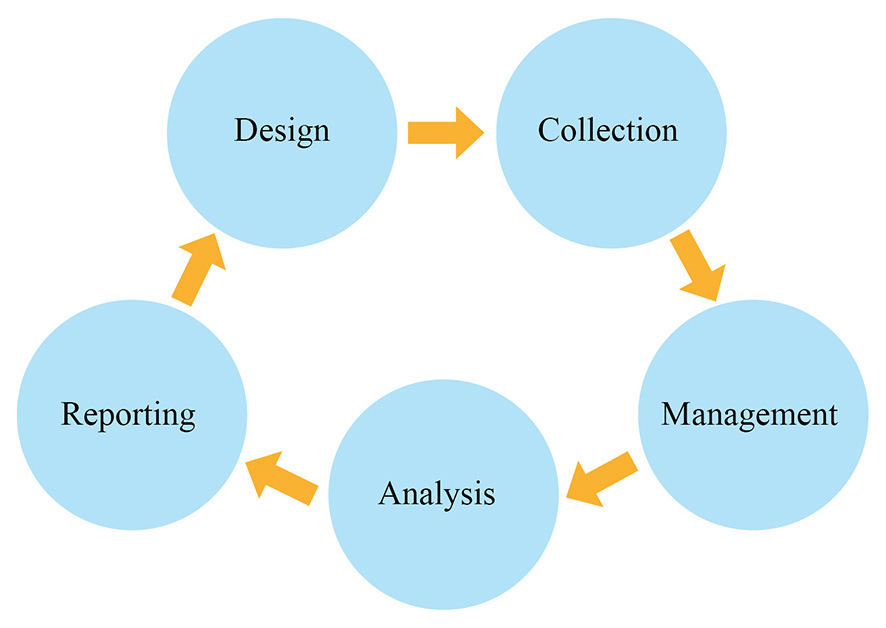
\includegraphics[width=0.75\textwidth]{literature/img/5stage.jpg}
	\caption{The 5 stages of survey research}
	\label{fig:literature:5stages}
	\end{figure}

	The authoring languages studied are focused on one or more stages of the survey research cycle. For instance, \gls{triples} and \gls{ddi} pay special attention to analysis and reporting stages since they provide structures that permit exporting the data collected for a questionnaire as well as its associated meta data. 
	In contrast, \gls{qdl} is best suited to address the design stage since it is built as part of a project to develop a tool for documenting questionnaire specifications \cite{man:bethlehem02}. 

	Whilst \gls{sss}, although was built to facilitate the creation of intuitive interfaces for supporting the design stage, it is more adequate to drive the collection stage given its formalism to describe expressions which offers more advantages than its counterparts and permits reducing the number of validations that have to be carried out before executing a questionnaire.